\section{Learning to Classify IC{\scriptsize s}}
\label{sec:model}

Beyond the observational study reported in Section~\ref{sec:preliminary}, we
propose an approach to identify influential changes on-the-fly. The objective
is to classify, when a change is being submitted, whether it should be
considered with care as it could be influential or not (i.e., binary prediction: IC or non-IC). Note that this approach does not classify a commit into specific IC types described in Section~\ref{sec:preliminary}.
To that end, the approach
leverages Machine Learning (ML) techniques. In our study, the learning process
is performed based on the dataset yielded by the systematic post-mortem
analysis and whose labels were manually confirmed. In this section, we describe
the features that we use to build classifiers as well as the quantitative
assessment that was performed.

\subsection{Machine Learning Features for ICs}

A change submitted to a project repository contains information on what the
change does (in commit messages), files touched by the change, the number of
edits performed by the change and so on. Based on the experience gathered
during the manual analysis of influential changes in
Section~\ref{sec:preliminary}, we extract a number of features to feed the ML
algorithms. The summary of features we used in this study is listed in Table~\ref{tab:learningfeatures} and the following sections describe more details on the features.




\subsubsection{Structural features.}
First we consider common metrics that provide hints on structural
characteristics of a change.
These metrics include (1) the number of files simultaneously changed in a single
commit, (2) the number of lines added to the program repository by the 
commit and (3) the number of lines removed from the code base.


\subsubsection{Natural language terms in commit messages.} During the
observational study, we noted that commit messages already contain good hints
on the importance of the change that they propose. We use the {\it Bag-of-
words}~\cite{lewis:ecml:1998} model to compute the frequency of occurrence of
words and use it as a feature. In addition, we noted that developers may be
emotional in the description of the change that they propose. Thus, we also
compute the subjectivity and polarity of commit messages based on {\em
sentiment analysis}~\cite{hu_opinion_2006,ohana_opinion_2009,
liu_sentiment_2010,thelwall_sentiment_2010} techniques.

\begin{table}[!t]
    \caption{Features used in learning a prediction model for ICs.}
    \label{tab:learningfeatures}
    \centering
\resizebox{\linewidth}{!}{
\begin{tabular}{l|l|c|l}
Category & Feature & Type & Description \\ \hline
\multirow{3}{*}{Structural} & \# files & Numeric & Number of files simultaneously changed in a single commit. \\ \cline{2-4}

& \# l-added & Numeric & Number of lines added to the program repository by the commit. \\ \cline{2-4}

& \# l-removed & Numeric & number of lines removed from the code base by the commit. \\ \hline

\multirow{3}{*}{NL Terms} & \# freq($token_{i}$) & Numeric & Frequency of occurrence of $token_{i}$. The number of features varies for each project.\\ \cline{2-4}

& Subjectivity & Boolean & Binary value indicating whether a commit message is subjective or objective. \\ \cline{2-4}

& Polarity & Boolean & Binary value indicating whether a commit message is negative or positive \\ \hline

\multirow{4}{*}{Co-change} & Max. PageRank & Numecric & Maximum value of PageRank for each file in a commit. \\ 
& & & PageRank is computed in a co-change graph built on a revision history of a project. \\ \cline{2-4}

 & Min. PageRank & Numeric & Minimum value of PageRank for each file in a commit. \\ \cline{2-4}
 

  & Betweeness Centrality & Numeric & Delta of the \textit{betweenness centrality} values of files between current and previous commits. \\ \cline{2-4}
  
  & Closeness Centrality & Numeric & Delta of the \textit{closeness centrality} values of files between current and previous commits. \\

\bottomrule

\end{tabular}
}

\end{table}

\begin{table*}[!t]
    \caption{Performance comparison using Na\"{i}ve Bayes and Random Forest classifiers.}
    \label{tab:f-measure}
    \centering
\resizebox{\linewidth}{!}{
\begin{tabular}{c | c | c c c c c c c c | c}
& {\bf Algorithm} & {\bf Commons-} & {\bf Commons-} & {\bf Commons-} & {\bf Commons-} & {\bf Commons-} & {\bf Commons-} & {\bf Commons-} & {\bf Storm}  & {\bf Average}\\

&  & {\bf codec} & {\bf collections} & {\bf compress} & {\bf csv} & {\bf io} & {\bf lang} & {\bf math} &  & \\


\toprule

{\bf F-Measure}
& NB & 95.1 & 92.9 & 91.5 & 84.2 & 98.5 & 89.2 & 94.3 & 86.1 & 91.5 \\
{\bf (Influential Class)}
& RF & 97.4 & 96.4 & 98.2 & 77.8 & 97.0 & 95.0 & 99.1 & 97.8 & 94.8 \\
\midrule
{\bf F-Measure}
& NB & 93.5 & 87.5 & 83.9 & 92.7 & 98.1 & 79.5 & 92.6 & 86.5 & 89.3 \\
{\bf (Non Influential Class)}
& RF & 97.0 & 93.9 & 97.1 & 90.5 & 96.3 & 92.9 & 98.9 & 97.5 & 95.5 \\

\bottomrule

\end{tabular}
}

\end{table*}

\subsubsection{Co-change impact.}
Finally, we consider that the frequency to which a pair of files are changed
together can be an indication of whether a given change commit affecting both
files (or not) is influential.
% Figure~\ref{fig:co-change} illustrate a {\it co-change}~\cite{Beyer05} graph for
% all files from the {\tt Commons-CSV} project.
In our experiments, for each commit, we build a co-change graph of the entire
project taking into account the history of changes until the time of that
commit. Then, considering files that are actually touched by the
change commit, we extract common network metrics.

% \begin{figure}[h!]
%     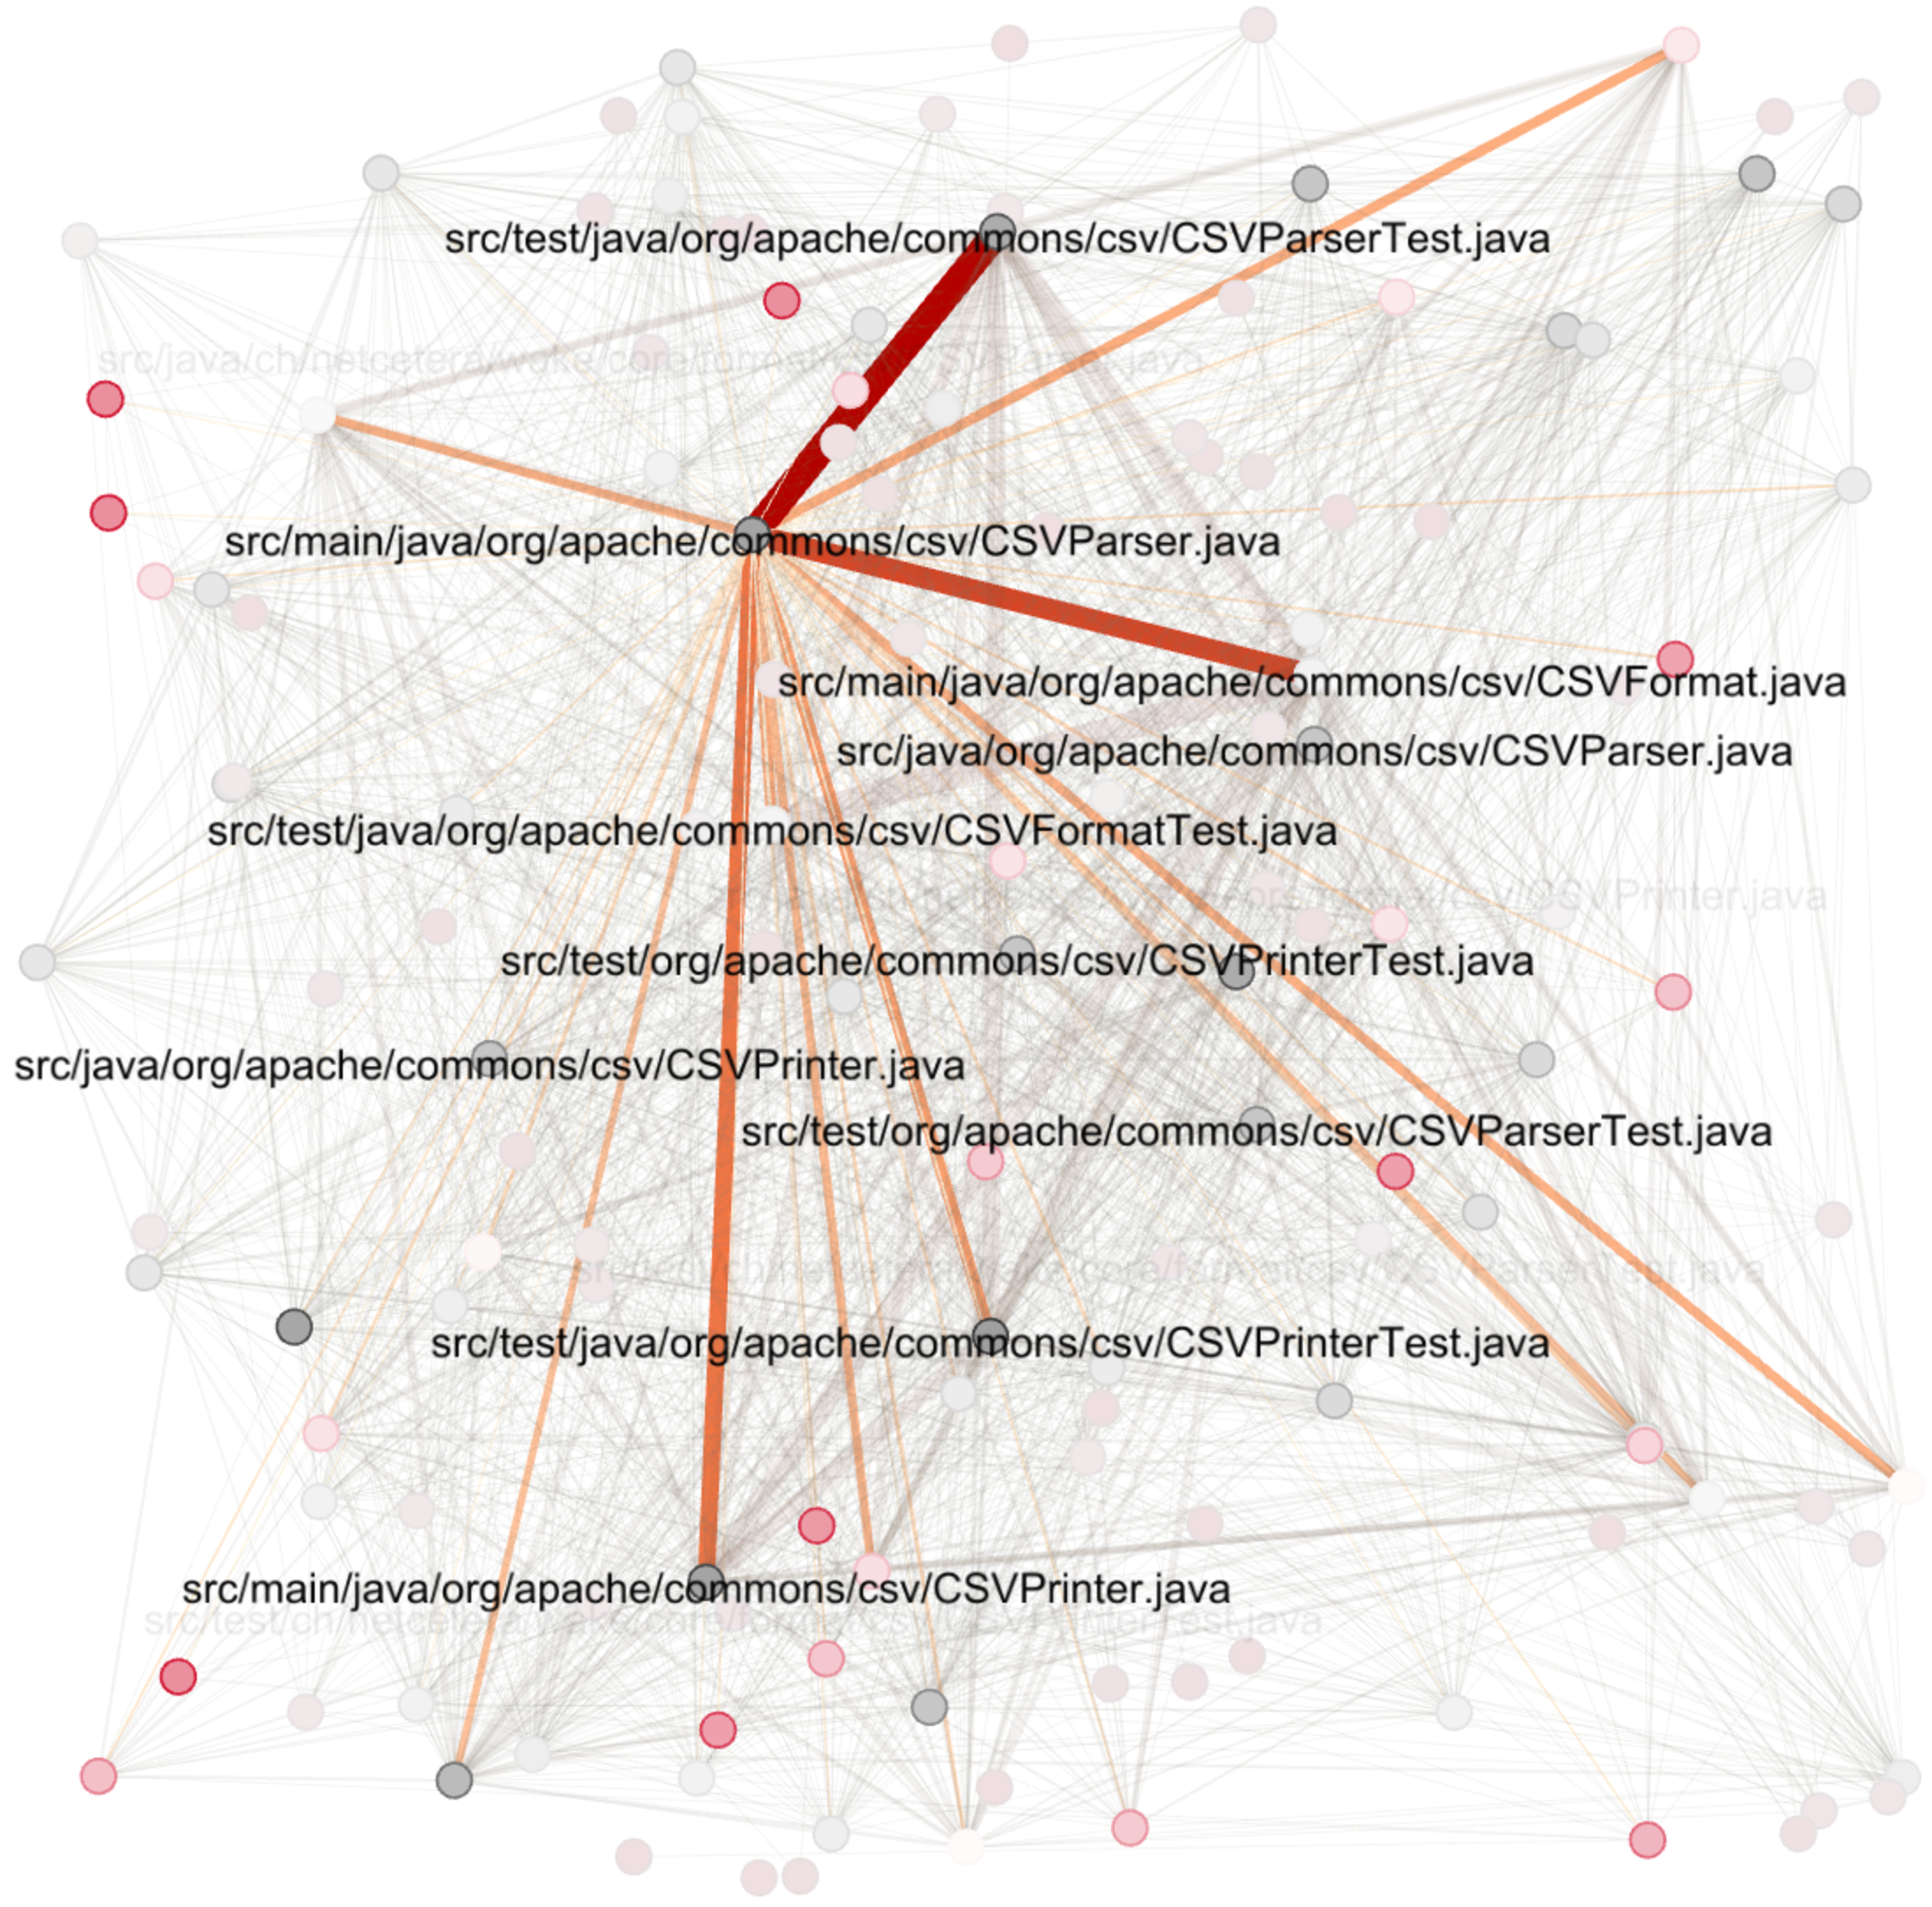
\includegraphics[width=0.9\linewidth]{fig/cochange-graph.pdf}
%     \caption{Co-Change graph of all files in the {\tt Commons-CSV} project.
%     Each node represents a file and the thickness of each edge corresponds to
%     the weight of co-change among two files.}
%     \label{fig:co-change}
% \end{figure}

\textbf{PageRank}~\cite{Brin98} is a link analysis algorithm for ``measuring'' the importance of
an element, namely a page, in a hyperlinked set of documents such as the World Wide Web. In our study, this metric is used for computing the likelihood that a file is changed together with other files.
Considering a co-change graph as a linked set, we extract PageRank values for all files. When a commit change is
applied, the co-change graph can be changed and then we re-compute new PageRank values. We take (newly computed) PageRank values of changed files in a commit after applying the commit to the co-change graph. Among the values, the minimum and maximum are used for features.

% We build a feature vector taking into
% account these changes on the minimum and maximum PageRank values.

\textbf{Centrality} metrics are commonly used in social network analysis to determine influential people
or to identify key nodes in networks. We use these metrics to represent how much a file is well-connected with other changed files in this study. 
In our experiments, we focus on computing 
{\it betweenness centrality}~\cite{freeman07}
and {\it closeness centrality}~\cite{Sabidussi66} metrics for all files associated with a commit change.
We compute betweenness and closeness centrality metrics of each file involved in a commit. After taking the sum of each centrality metric for all files in the commit, 
we then compute the delta of the sum between the current and previous commits. 
The delta of each centrality metric is used as our feature.

% We build features by computing

% the deltas in the sum of centrality metrics between the
% metrics computed for files involved in previous commits and for
% files involved in current commit.



\subsection{Influential Change Classification}
\label{sec:classresults}

In this section, we present the parameters of our Machine Learning classification
experiments for predicting influential changes. In these experiments, we assess
the quality of our features for accurately classifying influential
changes. We perform tests with two
popular classifiers, the Na\"{i}ve Bayes~\cite{lewis:ecml:1998,mlbook}
and Random Forest~\cite{breiman_random_2001}.

% In the process of our validation tests, we are interested in assessing:

% \begin{itemize}
%   \item Whether the connectedness on the co-change graph correlated with a probability
%   for a relevant change to be an IC;
%   \item If natural language information in commit messages are indicative of ICs;
%   \item If structural information of changes are indicative of ICs;
%   \item Whether combinations of features is best for predicting ICs;
%   \item If our approach can discover ICs beyond the types of changes
%   discovered with post-mortem analysis.
% \end{itemize}

In the process of our validation tests, we are interested in assessing: 1)
Whether connectivity on co-change graphs correlates with a probability
for a relevant change to be an IC; 2) If natural language information in
commit messages are indicative of ICs; 3) If structural information of changes
are indicative of ICs; 4) Whether combinations of features is best for
predicting ICs; 5) If our approach can discover ICs beyond the types of
changes discovered with post-mortem analysis.

% In the process of our validation tests, we answer the following questions:

% \begin{itemize}
%   % \item RQ1: Is our prediction scheme highly dependent on the classification algorithm?
%   \item Q1: Is the connectedness on the co-change graph correlated with a probability
%   for a relevant change to be an IC?
%   \item Q2: Is natural language information in commit message indicative of ICs?
%   \item Q3: Is structural information of changes indicative of ICs?
%   %\item RQ4: Are early changes more likely to be ICs?\dongsun{optional} \tb{This might be beyond the scope of this study... If the paper passes, we can make a journal paper with that}
%   \item Q4: What combinations of features is best for predicting ICs?
%   \item Q5: Can our approach discover ICs beyond the types of changes
%   discovered with post-mortem analysis?
% \end{itemize}

\subsubsection{Experiment Setup.}\label{sec:experiment}
To compute the feature vectors for training the classifiers, we used 
a high-performance computing system~\cite{VBCG_HPCS14} to run parallel tasks for
building co-change graphs for the various project subjects. After extracting the
feature metrics, we preprocessed the data and ran ten-fold cross validation
tests to measure the performance of the classification.

\textbf{Preprocessing.}
Influential software changes likely constitute a small subset of all changes
committed in the project repositories. Our manual analysis yielded very few
influential changes leading to a problem of imbalanced datasets in the training
data.
Since we try to identify influential changes, which constitute the minority
classes and learning algorithms are not adapted to imbalanced datasets, we use oversampling
techniques to adjust the class distribution. In our experiments, we leverage
the Synthetic Minority Over-sampling Techniques (SMOTE)~\cite{al.2002}.

\textbf{Evaluation Measures.}
To quantitatively evaluate the performance of our approach for predicting influential changes,
we used standard metrics in ML, namely Precision, Recall and
F-measure~\cite{mlbook,kim_classifying_2008,stat2}. {\bf Precision} quantifies the effectiveness of our machine learning-based approach to point to changes that are actually influential. {\bf Recall} on the other hand explores the capability of our approach to identify most of the influential changes in the commits set. Finally, we compute the {\bf F-measure}, the harmonic mean between Recall and Precision. We consider that both Precision and Recall are equally important and thus, they are equally weighted in the computation of F-measure.
 % in Equation (1).
% \begin{equation}
%     F-measure=F_1=2 \cdot \frac{Precision \cdot Recall}{Precision + Recall}
% \end{equation}
% \daoyuan{We can drop this when running out of space.}
% \begin{itemize}
% \itemsep0em 
% \item {\bf Precision} quantifies the effectiveness of our machine learning-based approach to point to
%     changes that are actually influential.
% \item {\bf Recall} on the other hand explores the capability of our approach to identify most of the influential changes in the commits set.
% \item Finally, we compute the {\bf F-measure}, the harmonic mean between Recall and Precision. We consider that
%     both Precision and Recall are equally important and thus, they are equally weighted in the computation of F-measure in Equation (1) 
%     \begin{equation}
%         F-measure=F_1=2 \cdot \frac{Precision \cdot Recall}{Precision + Recall}
%     \end{equation}
% \end{itemize}


\subsubsection{Assessment Results.}
In the following paragraphs, we detail the classification results for
influential changes using ten-fold cross validation on labeled
data. In addition, we present experimental results of the performance of the classification models with new dataset labeled based on developer accepted definitions of influential challenges.


% \paragraph{Ten-Fold Cross Validation}
Cross validation is a common model validation in statistics to
assess how the results of a statistical analysis will generalize to an
independent data set. In machine learning experiments, it is common practice to
rely on {\it k-fold} cross validation where the test is performed {\it k} times,
each time testing on a $k^{th}$ portion of the data. We perform ten-fold cross
validation on the labeled dataset built in Section~\ref{sec:preliminary}.

In the first round of experiments, we built feature vectors with all
features considered in our study. We then built classifiers using Na\"{i}ve
Bayes and Random Forest. Table~\ref{tab:f-measure} depicts the F-measure
performance in ten-fold cross validation for the two algorithms. Although
Random Forest performs on average better than Na\"{i}ve Bayes, this difference
is relatively small.




% \begin{center}
% \setlength{\fboxsep}{5pt}%
% \Ovalbox{%
% \begin{minipage}{.42\textwidth}
% \begin{center}
%     {{\bf RQ1:}\it Our prediction model, with the features of
%     influential changes, is not significantly dependent on the classification algorithm 
%     as suggested by their average F-measure performances (94.8\% and 91.5\% for
%     the influential class).
%     }
% \end{center}
% \end{minipage}}
% \end{center}

% Figure~\ref{fig:roc} illustrates the performance of our binary classifier for the Influential class,
% for the different projects using Random Forest classification algorithm with the combination of all features. The Area Under Curve (AUC) metric
% values are all higher than 0.9 for all projects, implying a very performant prediction model.

% \begin{figure}[h!] 
%     \centering 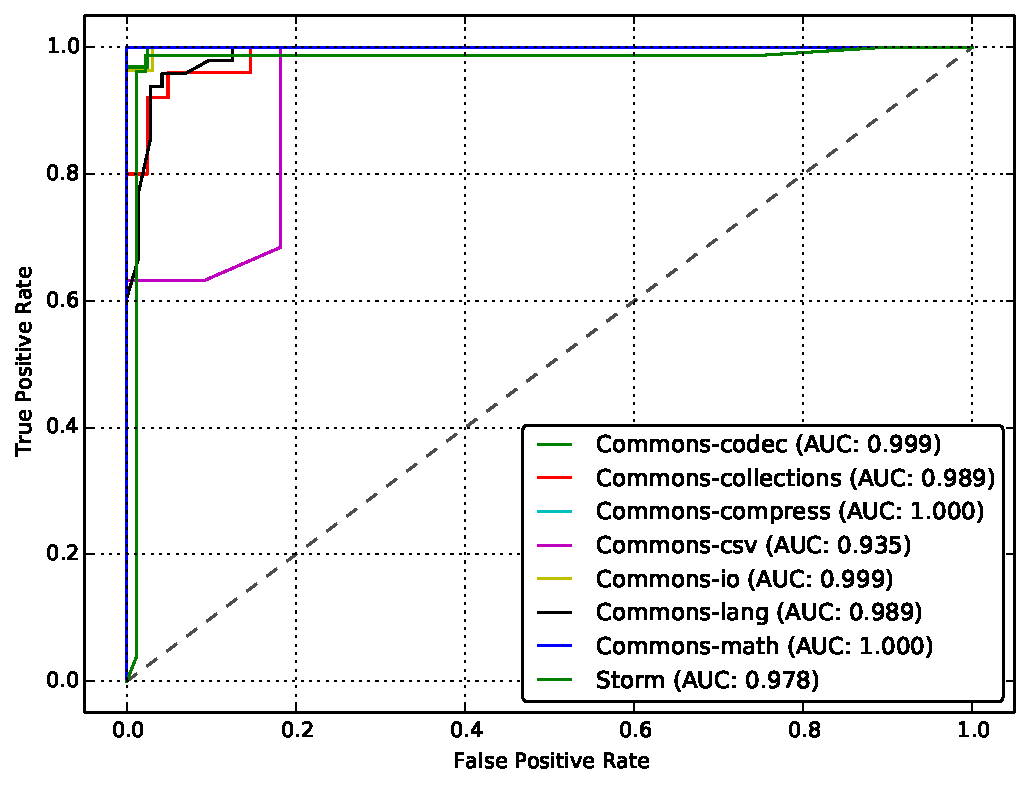
\includegraphics[width=0.9\linewidth]{fig/roc.pdf}
% \caption{Receiver Operating Characteristic curves for classification of influential changes in test projects}
% \label{fig:roc}
% \end{figure}

Table~\ref{tab:ten-fold-rf} details the validation results with Random Forest for different combinations 
of feature groups for the experiments.
We considered separately features relevant to co-change metrics, commit messages written in a natural
language, and the structural information of changes. We
also combined those type of features to assess the potential performance
improvement or deterioration.

\begin{table}[h!]
    \caption{Ten-fold cross validation on influential changes using 
    Random Forest with different metrics combinations. 
    CC: co-change features. NL: natural language terms on commit messages.
    SI: structural features.}
    \label{tab:ten-fold-rf}
    \centering
\resizebox{0.5\linewidth}{!}{
\begin{tabular}{l l | c c c | c c c}
  \multirow{2}{*}{\bf Project Name} & 
  \multirow{2}{*}{\bf Metrics} &
  \multicolumn{3}{c|}{\bf Influential Class} & 
  \multicolumn{3}{c}{\bf Non-Influential Class} \\
  & & Precision & Recall & F-Measure & Precision & Recall & F-Measure \\

\toprule

{\tt Commons-codec}
& \highlight CC & 97.5 & 97.5 & \highlight 97.5 & 96.9 & 96.9 & 96.9 \\
& NL & 100.0 & 92.5 & 96.1 & 91.4 & 100.0 & 95.5 \\
& SI & 81.0 & 85.0 & 82.9 & 80.0 & 75.0 & 77.4 \\
& CC NL & 100.0 & 95.0 & 97.4 & 94.1 & 100.0 & 97.0 \\
& CC SI & 95.0 & 95.0 & 95.0 & 93.8 & 93.8 & 93.8 \\
& NL SI & 100.0 & 95.0 & 97.4 & 94.1 & 100.0 & 97.0 \\
& ALL & 100.0 & 95.0 & 97.4 & 94.1 & 100.0 & 97.0 \\
\midrule
{\tt Commons-}
& CC & 90.5 & 92.7 & 91.6 & 87.5 & 84.0 & 85.7 \\
{\tt collections}
& NL & 94.9 & 90.2 & 92.5 & 85.2 & 92.0 & 88.5 \\
& SI & 80.4 & 90.2 & 85.1 & 80.0 & 64.0 & 71.1 \\
& CC NL & 97.3 & 87.8 & 92.3 & 82.8 & 96.0 & 88.9 \\
& CC SI & 86.7 & 95.1 & 90.7 & 90.5 & 76.0 & 82.6 \\
& NL SI & 95.1 & 95.1 & 95.1 & 92.0 & 92.0 & 92.0 \\
& \highlight ALL & 95.2 & 97.6 & \highlight 96.4 & 95.8 & 92.0 & 93.9 \\
\midrule
{\tt Commons-}
& CC & 92.9 & 96.3 & 94.5 & 94.1 & 88.9 & 91.4 \\
{\tt compress}
& NL & 100.0 & 96.3 & 98.1 & 94.7 & 100.0 & 97.3 \\
& SI & 89.7 & 96.3 & 92.9 & 93.8 & 83.3 & 88.2 \\
& CC NL & 100.0 & 96.3 & 98.1 & 94.7 & 100.0 & 97.3 \\
& CC SI & 87.1 & 100.0 & 93.1 & 100.0 & 77.8 & 87.5 \\
& \highlight NL SI & 100.0 & 100.0 & \highlight 100.0 & 100.0 & 100.0 & 100.0 \\
& ALL & 96.4 & 100.0 & 98.2 & 100.0 & 94.4 & 97.1 \\
\midrule
{\tt Commons-csv}
& CC & 40.0 & 36.4 & 38.1 & 65.0 & 68.4 & 66.7 \\
& NL & 100.0 & 63.6 & 77.8 & 82.6 & 100.0 & 90.5 \\
& \highlight SI & 100.0 & 81.8 & \highlight 90.0 & 90.5 & 100.0 & 95.0 \\
& CC NL & 100.0 & 54.5 & 70.6 & 79.2 & 100.0 & 88.4 \\
& CC SI & 66.7 & 54.5 & 60.0 & 76.2 & 84.2 & 80.0 \\
& NL SI & 100.0 & 72.7 & 84.2 & 86.4 & 100.0 & 92.7 \\
& ALL & 100.0 & 63.6 & 77.8 & 82.6 & 100.0 & 90.5 \\
\midrule
{\tt Commons-io}
& CC & 93.9 & 93.9 & 93.9 & 92.6 & 92.6 & 92.6 \\
& \highlight NL & 100.0 & 97.0 & \highlight 98.5 & 96.4 & 100.0 & 98.2 \\
& SI & 82.5 & 100.0 & 90.4 & 100.0 & 74.1 & 85.1 \\
& \highlight CC NL & 100.0 & 97.0 & \highlight 98.5 & 96.4 & 100.0 & 98.2 \\
& CC SI & 94.1 & 97.0 & 95.5 & 96.2 & 92.6 & 94.3 \\
& \highlight NL SI & 100.0 & 97.0 & \highlight 98.5 & 96.4 & 100.0 & 98.2 \\
& ALL & 97.0 & 97.0 & 97.0 & 96.3 & 96.3 & 96.3 \\
\midrule
{\tt Commons-lang}
& CC & 86.5 & 88.9 & 87.7 & 82.6 & 79.2 & 80.9 \\
& NL & 94.4 & 93.1 & 93.7 & 89.8 & 91.7 & 90.7 \\
& SI & 72.2 & 79.2 & 75.5 & 63.4 & 54.2 & 58.4 \\
& \highlight CC NL & 95.8 & 95.8 & \highlight 95.8 & 93.8 & 93.8 & 93.8 \\
& CC SI & 91.9 & 94.4 & 93.2 & 91.3 & 87.5 & 89.4 \\
& NL SI & 98.5 & 93.1 & 95.7 & 90.4 & 97.9 & 94.0 \\
& ALL & 97.1 & 93.1 & 95.0 & 90.2 & 95.8 & 92.9 \\
\midrule
{\tt Commons-math}
& CC & 95.4 & 96.3 & 95.9 & 95.7 & 94.7 & 95.2 \\
& \highlight NL & 100.0 & 100.0 & \highlight 100.0 & 100.0 & 100.0 & 100.0 \\
& SI & 76.3 & 80.6 & 78.4 & 76.1 & 71.3 & 73.6 \\
& \highlight CC NL & 100.0 & 100.0 & \highlight 100.0 & 100.0 & 100.0 & 100.0 \\
& CC SI & 96.4 & 98.1 & 97.2 & 97.8 & 95.7 & 96.8 \\
& NL SI & 100.0 & 98.1 & 99.1 & 97.9 & 100.0 & 98.9 \\
& ALL & 100.0 & 98.1 & 99.1 & 97.9 & 100.0 & 98.9 \\
\midrule
\midrule
{\tt Spring-}
& \highlight NL & 96.2 & 90.9 & \highlight 93.5 & 84.6 & 93.2 & 88.7 \\
{\tt framework}
& SI & 75.8 & 88.2 & 81.5 & 68.3 & 47.5 & 56.0 \\
& NL SI & 96.0 & 86.4 & 90.9 & 78.6 & 93.2 & 85.3 \\
\midrule
{\tt Storm}
& CC & 97.7 & 95.5 & 96.6 & 95.1 & 97.5 & 96.2 \\
& NL & 97.8 & 98.9 & 98.3 & 98.7 & 97.5 & 98.1 \\
& SI & 90.0 & 80.9 & 85.2 & 80.7 & 89.9 & 85.0 \\
& CC NL & 97.8 & 97.8 & 97.8 & 97.5 & 97.5 & 97.5 \\
& CC SI & 97.7 & 95.5 & 96.6 & 95.1 & 97.5 & 96.2 \\
& \highlight NL SI & 98.9 & 98.9 & \highlight 98.9 & 98.7 & 98.7 & 98.7 \\
& ALL & 97.8 & 97.8 & 97.8 & 97.5 & 97.5 & 97.5 \\
\midrule
\midrule
{\tt Wildfly}
& NL & 93.7 & 98.4 & 96.0 & 98.0 & 92.6 & 95.2 \\
& SI & 78.7 & 82.3 & 80.5 & 79.0 & 75.0 & 77.0 \\
& \highlight NL SI & 96.0 & 99.2 & \highlight 97.6 & 99.0 & 95.4 & 97.2 \\

\bottomrule
\end{tabular}
}

\end{table}

Co-change metrics, which are the most tedious to extract (hence missing from two projects in Table~\ref{tab:ten-fold-rf} due to too large graphs)
histories, allow to yield an average performance of 87.7\% precision, 
87.5\% recall, and 87.6\% F-measure.

% \begin{center}
% \setlength{\fboxsep}{5pt}%
% \Ovalbox{%
% \begin{minipage}{.42\textwidth}
% \begin{center}
%     {{\bf Q1:}\it Co-change metrics allow to successfully predict 
%     influential changes with an average 87.6\% F-measure.
%     }
% \end{center}
% \end{minipage}}
% \end{center}

Natural language terms in commit messages also allow yielding an average
performance of 94.9\% precision, 94.4\% recall, and 94.4\% F-measure
for the influential change class on average.

% \begin{center}
% \setlength{\fboxsep}{5pt}%
% \Ovalbox{%
% \begin{minipage}{.42\textwidth}
% \begin{center}
%     {{\bf Q2:}\it Features based on terms in commit messages
%         can predict influential changes with high precision 
%         (average of 94.9\%) and recall (average of 94.4\%).
%     }
% \end{center}
% \end{minipage}}
% \end{center}

Our experiments also revealed that structural features of changes yield the
worst performance rates, although those performances reached 80.5\%
F-measure on average. For some projects, however, these metrics lead to a
performance slightly above 50\% (random baseline performance).

% \begin{center}
% \setlength{\fboxsep}{5pt}%
% \Ovalbox{%
% \begin{minipage}{.42\textwidth}
% \begin{center}
%     {{\bf Q3:}\it Structural features can be leveraged to 
%     successfully predict influential changes with an average F-measure performance of 80.5\%.
%     }
% \end{center}
% \end{minipage}}
% \end{center}

The performance results shown in Table~\ref{tab:ten-fold-rf} also highlight
the fact that, on average, combining different features contributes to improving
the performance of influential change classification. Combining co-change and
natural language terms in commit messages achieves on average a precision, recall and
F-measure performance of 95.6\%, 94.5\%, and 94.5\% respectively.
Similarly, combining co-change and structural features shows the F-measures at
90.1\% on average. Combinations of natural language and structural information
show 95.6\% F-measure. Finally, combining all features leads to an average
performance of 96.1\% precision, 94.9\% recall, and 95.2\% F-measure. However,
no feature combination achieves the best performance in every project, possibly
suggesting these features are specific to projects.

Figure~\ref{fig:auroc} further shows graphically the Area Under the Receiver Operating Characteristic (AUROC) for the predictors including all features. Overall, we note that the performance of the classifiers is high.

\begin{figure}
\centering
	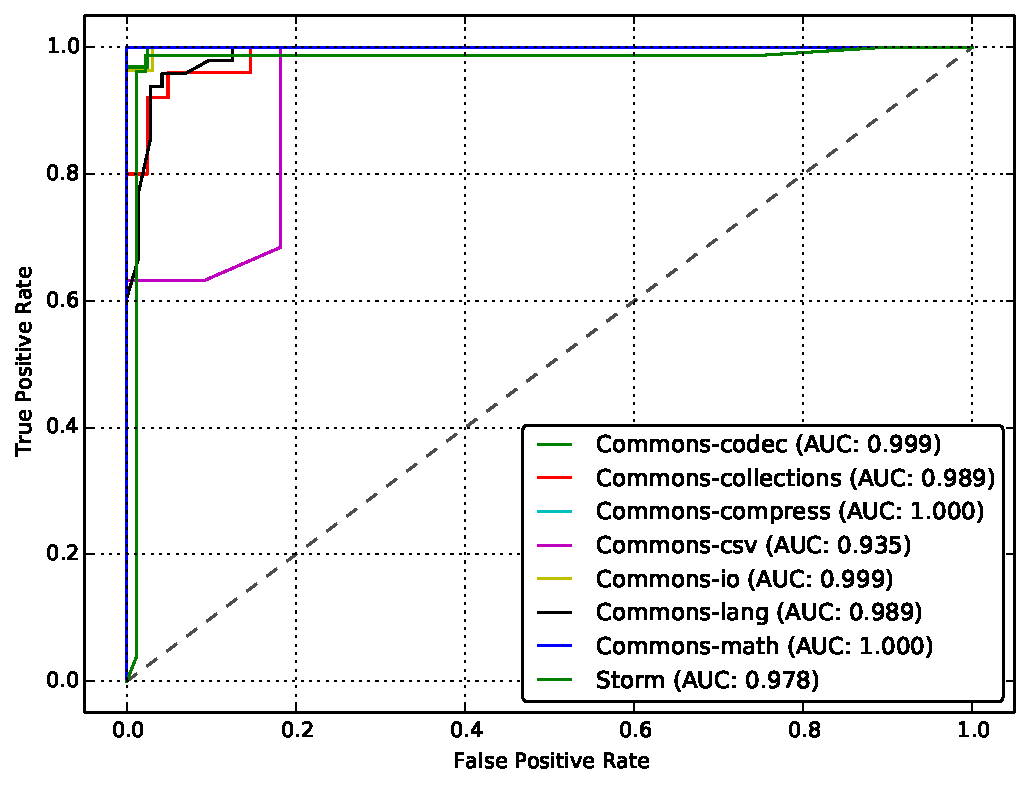
\includegraphics[width=0.8\linewidth]{fig/roc}
	\caption{Receiver Operating Characteristic for predictors in all 10 projects.}
	\label{fig:auroc}
\end{figure}
% \begin{center}
% \setlength{\fboxsep}{5pt}%
% \Ovalbox{%
% \begin{minipage}{.42\textwidth}
% \begin{center}
%     {{\bf Q4:}\it Overall, combining features often achieves a better
%     prediction performance than individual feature groups. 
%         For example, combining all features showed 96.1\% precision, 94.9\%
% recall, and 95.2\% F-measure on average.
%     }
% \end{center}
% \end{minipage}}
% \end{center}


\subsubsection{Generalization of Influential Change Features.}
In previous experiments, we have tested the machine learning classifier with
influential change data labeled based on three specific criteria (changes that
fix controversial/popular issues, isolated changes and changes referenced by other changes).
These categories are however strictly related to our initial intuitions for collecting influential
changes in a post-mortem analysis study. There are likely many influential changes that do not
fit into those categories. Our objective is thus to evaluate whether the \textit{features} that we
use for classification of influential changes are still relevant in the wild. In other words, the experiment aims at figuring out the generalizability of the features rather than the models used in previous experiments.



We randomly sample a significant set of changes within our dataset of 10 projects commits. 
Out of the \numChanges commits from the dataset, we randomly consider 381 commits (i.e., the
exact number provided by the Sample Size
Calculator\footnote{\url{http://www.surveysystem.com/sscalc.htm}} using
95\% for the confidence level and 5 for the confidence interval).

Again we manually label the data based on the categories of influential changes approved by developers (cf. Section~\ref{subsec.opencard}).
We cross check our labels among authors and perform ten-fold cross validation using the same features presented in Section~\ref{sec:experiment} for
influential change classification. The results are presented in Table~\ref{tab:ten-fold-rf-random}.

\begin{table}[h!]
\caption{Ten-fold cross validation on randomly sampled
and then manually labelled data. We show results considering all features (NL
and SI features in the case of {\tt Spring-framework} and {\tt Wildfly}
because of missing CC features).}

\label{tab:ten-fold-rf-random}
    \centering
\resizebox{0.9\linewidth}{!}
{
\begin{tabular}{l | c c c | c c c}
  \multirow{2}{*}{\bf Project Name} & 
  \multicolumn{3}{c|}{\bf Influential Class} & 
  \multicolumn{3}{c}{\bf Non-Influential Class} \\
  & Precision & Recall & F-Measure & Precision & Recall & F-Measure \\

\toprule

{\tt Commons-codec}
& 100.0 & 88.9 & 94.1 & 87.5 & 100.0 & 93.3 \\
{\tt Commons-collections}
& 100.0 & 88.9 & 94.1 & 83.3 & 100.0 & 90.9 \\
{\tt Commons-compress}
& 0.0 & 0.0 & 0.0 & 66.7 & 100.0 & 80.0 \\
% {\tt Commons-csv}
% % & 100.0 & 63.6 & 77.8 & 82.6 & 100.0 & 90.5 \\
% &  &  &  &   &   &  \\
{\tt Commons-io}
& 86.7 & 86.7 & 86.7 & 75.0 & 75.0 & 75.0 \\
{\tt Commons-lang}
& 97.3 & 90.0 & 93.5 & 85.2 & 95.8 & 90.2 \\
{\tt Commons-math}
& 100.0 & 31.6 & 48.0 & 71.1 & 100.0 & 83.1 \\
{\tt Spring-framework}
& 97.5 & 96.9 & 97.2 & 91.7 & 93.2 & 92.4 \\
{\tt Storm}
& 100.0 & 88.2 & 93.8 & 88.2 & 100.0 & 93.8 \\
{\tt Wildfly}
& 100.0 & 96.4 & 98.2 & 95.8 & 100.0 & 97.8 \\

\bottomrule
\end{tabular}
}

\end{table}

The precision of ten-fold cross validation for influential changes is on average 86.8\% while the average recall
is 74\%. These results suggest that overall, the features provided in our
study are effective even in the wild. For some projects, the performance is
especially poor, mainly because 1) their training data is limited ({\tt Commons-CSV}
has only one labeled influential change, making it infeasible to even oversample; thus
no results are available in the table), 2) currently, we do not take into account some features
of influential changes related to documentation. Developers have already brought up this aspect in the survey.

%
%Finally, based on our labelled data, we built a classifier for predicting
%influential changes in the wild, i.e., testing on all commit changes of a
%project.
%We then manually assessed the predicted influential changes. With this
%experiment we could validate the capability of our approach to perform in the
%wild and investigate whether our features allow to discover
%influential changes beyond the scope of those that we have identified in the
%post-mortem observational study.
%
%We ran the experiments on {\tt Commons-csv} and {\tt Commons\-codec} as they were
%the top two projects with the highest rates of labelled influential change
%compared to the total number of commit changes in their project repositories.
%For each project, we sampled 20 predicted influential changes to manually check.
%In 60\% and 65\% of changes, respectively in {\tt Commons-csv} and {\tt Commons-codec}, 
%the prediction yielded was correct.
%
%Then, we compared the predicted influential changes in the wild with the
%influential changes used for training the classifiers. We thus found that our
%prediction model allowed to {\it discover} new influential changes outside the
%sets that could be found in our systematic analysis of
%Section~\ref{sec:preliminary}.
%
%In particular, the experiments of prediction in the wild for the {\tt
%Commons-csv} revealed commit {\it c7576ccd} as an example of typical influential
%changes.
%This change is a simple refactoring of an API name ($isEndOfLine \longrightarrow
%readEndOfLine$). With this refactoring, current and future users of the API will
%now realize that the API method is not just a test method. Such a change may lead 
%to an increase in the number of places this API is used.

% \begin{center}
% \setlength{\fboxsep}{5pt}%
% \Ovalbox{%
% \begin{minipage}{.42\textwidth}
% \begin{center}
%     {{\bf Q5:}\it With the features we collected, our prediction approach 
%     is likely to perform in the wild, i.e., beyond
%         the scope of influential changes found 
%         in the collected training dataset (from post-mortem observational study).
%     }
% \end{center}
% \end{minipage}}
% \end{center}


\subsubsection{Evaluation Summary.}

% From our evaluation results we have found out that:

% \begin{itemize}
% \itemsep0em 
%   \item Co-change metrics allow to successfully predict 
%     influential changes with an average 87.6\% F-measure;
%   \item Features based on terms in commit messages
%         can predict influential changes with high precision 
%         (average of 94.9\%) and recall (average of 94.4\%);
%   \item Structural features can be leveraged to 
%     successfully predict influential changes with an average F-measure performance of 80.5\%;
%   \item Overall, combining features often achieves a better
%     prediction performance than individual feature groups. 
%         For example, combining all features showed 96.1\% precision, 94.9\%
% recall, and 95.2\% F-measure on average;
%   \item With the features we collected, our prediction approach 
%     is likely to perform in the wild, i.e., beyond
%         the scope of influential changes found 
%         in the collected training dataset (from post-mortem observational study).
% \end{itemize}

From our evaluation results we have found that: 1) Co-change metrics allow
to successfully predict influential changes with an average 87.6\% F-measure;
2) Features based on terms in commit messages can predict influential changes
with high precision (average of 94.9\%) and recall (average of 94.4\%); 3)
Structural features can be leveraged to successfully predict influential
changes with an average F-measure performance of 80.5\%; 4) Overall, combining
features often achieves a better classification performance than individual
feature groups. For example, combining all features showed 96.1\% precision,
94.9\% recall, and 95.2\% F-measure on average; 5) With the features we
collected, our classification model has an acceptable performance in the wild, i.e.,
with different types of influential changes (beyond the ones we relied upon to infer
the features).
